В разделах \ref{chapter2/diploma-section-2-1} и \ref{chapter2/diploma-section-2-2} была показана возможность построения точного $D$-оптимального плана для описанной модели наблюдений. Конечной целью эксперимента является оценка параметров модели по полученным наблюдениям. Далее исследуем: при каких условиях и на сколько оценки, полученные по наблюдениям в условиях $D$-оптимального плана, точнее оценок, полученных в результате наблюдений в случайных точках?

\subsection{Модель наблюдений}
Рассмотрим модель наблюдений из \ref{chapter2/diploma-section-2-1}.
Пусть было проведено $N$ наблюдений. Модель наблюдений имеет вид:
\begin{gather} \label{numerical-experiment:model:start}
y_i = \theta_0 + \theta_1 x_{i1} + \theta_2 x_{i2} + \varepsilon(x^{(i)}), i = \overline{1, N}, N \ge 3; \\
E\{ \varepsilon(x^{(i)}) \} = 0, E\{ \varepsilon^{(i)}\ \varepsilon^{(j)} \} = 0, i \ne j; \\
D\{ \varepsilon(x^{(i)}) \} = d(x_{i1}, x_{i2}) > 0; \\
d(x_1, x_2) \ge \frac{\sigma^2}{3}(1 + x_1^2 + x_2^2);
\label{numerical-experiment:model:end}
\end{gather}
где $\varepsilon^{(i)}$ - случайные, неравноточные и некоррелированные ошибки с дисперсией $d(x_{i1}, x_{i2})$. $-1 \le x_{ij} \le 1$, $i=\overline{1,N}, j=\overline{1, 2}$.\\
Введём обозначения для точек:
\begin{equation}\label{numerical-experiment:plan-points}
x^{(1)}=(1, 1), x^{(2)}=(-1, 1), x^{(3)}=(-1, -1), x^{(4)}=(1, -1).
\end{equation}
И для значений дисперсии наблюдений в этих точках:
\begin{equation}
d(x^{(1)}) = d_1, d(x^{(2)}) = d_2, d(x^{(3)}) = d_3, d(x^{(4)}) = d_4.
\end{equation}
Согласно теореме \ref{main-theorem}, для указанной модели план
\begin{equation} \label{numerical-expetiment:plan-1}
\varepsilon_1^{0} = \left \{ 
\underset{\frac 1 3} {x^{(1)}},
\underset{\frac 1 3} {x^{(2)}},
\underset{\frac 1 3} {x^{(3)}}
\right \}
\end{equation}
является точным $D$-оптимальным, если
\begin{equation}\label{numerical-experiment:d-eq}
d(x_1, x_2) \ge \frac 1 4 (d_1 + d_3 + 2 d_1 x_1 - 2 d_3 x_2 - 2d_2 x_1 x_2 + (d_1 + d_2)x_1^2 + (d_2 + d_3)x_2^2).
\end{equation}

Далее в этом разделе рассмотрим случай, когда неравенство \ref{numerical-experiment:d} обращается в равенство:
\begin{equation}\label{numerical-experiment:d}
d(x_1, x_2) = \frac 1 4 (d_1 + d_3 + 2 d_1 x_1 - 2 d_3 x_2 - 2d_2 x_1 x_2 + (d_1 + d_2)x_1^2 + (d_2 + d_3)x_2^2).
\end{equation}

\subsection {Взвешенный метод наименьших квадратов для оценивания параметров}
Для оценивания параметров регрессионной модели в условиях теоремы Гаусса-Маркова применяет метод наименьших квадратов (МНК). Неравноточность наблюдений нарушает условия теоремы Гаусса-Маркова, поэтому для оценки параметров неравноточной регрессионной модели применяется другой метод -- взвешенный метод наименьших квадратов (взвешенный МНК). Взвешенный МНК является обобщением МНК, при котором каждое наблюдение учитывается с весом, обратно пропорциональным его дисперсии. 

Обозначим $X$ - матрица плана эксперимента, $y = (y_1, ..., y_N)^T$ -- вектор наблюдений, $\varepsilon = (\varepsilon_1, ..., \varepsilon_N)^T$ -- вектор случайных ошибок, $\theta = (\theta_0, \theta_1, \theta_2)^T$ -- вектор параметров. Тогда \eqref{numerical-experiment:model:start} можно переписать в матричной форме:
\begin{equation}
y = X\theta + \varepsilon.
\end{equation}
Обозначим $w = (w_1, ..., w_N)^T$ -- вектор весов наблюдений, где $w_i = D(x_{i1}, x_{i2}) = d(x_{i1}, x_{i2})$. Также обозначим $W = diag(w)$ -- диагональная матрица весов.
Тогда $\hat \theta$ -- оценка вектора параметров $\theta$ по взвешенному МНК имеет вид:
\begin{equation}
\hat \theta = (X^T W X)^{-1} X^T W y.
\end{equation}

Обоснование и свойства взвешенного МНК могут быть найдены, например, в \cite{aivazian}.

\subsection{Численный эксперимент}
Проведём численный эксперимент, чтобы понять, при каких условиях и на сколько $D$-оптимальный план эффективнее другого, случайного плана.
\subsubsection{Алгоритм проведения эксперимента.}
\begin{enumerate}
	\item \label{numerical-experiment:algo:loop:start}задать коэффициенты $\theta_0, \theta_1, \theta_2$ уравнения регрессии \eqref{numerical-experiment:model:start}, значения $d_1, d_2, d_3$ и, соответственно, функцию $d(x_1, x_2)$ согласно \eqref{numerical-experiment:d};
	\item задать количество наблюдений $N$, где $N$ кратно 3;
	\item сгенерировать матрицу плана эксперимента $X$ одним из способов:
		\begin{enumerate}
			\item $X = X_{optimal}$ -- согласно теореме о $D$-оптимальном плане, т.е. $N/3$ наблюдений в каждой из точек $x^{(1)}, x^{(2)}, x^{(3)}$;
			\item $X = X_{random}$ -- $N$ случайных точек из двумерного равномерного распределения $R^2[-1, 1]$;
		\end{enumerate}
	\item для $X$ сгенерировать вектор ошибок $\varepsilon$ с дисперсией $d(x_1, x_2)$;
	\item вычислить $y = X \theta + \varepsilon$;
	\item по взвешенному методу наименьших квадратов найти  $\hat \theta$ -- оценку вектора параметров $\theta$;
	\item \label{numerical-experiment:algo:loop:end} измерить точность оценки как среднеквадратическую ошибку: $e = \frac 1 3 \sum_{i=0}^{2} (\theta_i - \hat \theta_i)^2$. 
\end{enumerate}

Чтобы сделать результаты эксперимента более точными, описанный алгоритм повторяется $T$ раз и в качестве итоговой оценки точности берётся $\overline e = \frac 1 T \sum_{t=1}^{T} e_t$.

\subsubsection{Параметры эксперимента.}
Зададим конкретные значения параметров для проведения эксперимента.
\begin{enumerate}
	\item $\theta = (2, 5, 1)^T$;
	\item $d_1 = 6, d_2 = 4, d_3 = 2$;
	\item $N \in \{3, 6, ..., 24, 27\}$;
	\item $T = 5$.
\end{enumerate} 

\subsubsection{Реализация эксперимента.}
Для реализация описанного эксперимента была написана программа на языке программирования \textit{Python} с использованием пакетов \textit{NumPy}, \textit{SciPy}, \textit{scikit-learn} \cite{scikit-learn}. Исходный код программы приведён в приложении \ref{appendix:heteroscedastic_experiment}

\subsubsection{Результаты эксперимента.}
Рассмотрим график \ref{fig:heteroscedastic-experiment} изменения средней квадратичной ошибки оценок в зависимости от числа проведённых наблюдений. Закрашенная область соответствует $\overline e$ с учётом стандартного отклонения $\overline r$. Синяя линяя соответствует оптимальному плану, оранжевая -- случайному.

Видно, что $D$-оптимальный план эксперимента позволяет точно оценить параметры модели уже при $N=3$, в то время как случайный план является крайне неточными при $N < 9$. При $N > 9$ оба подхода дают почти одинаково точный результат.

\begin{figure}[h]
	\centering
	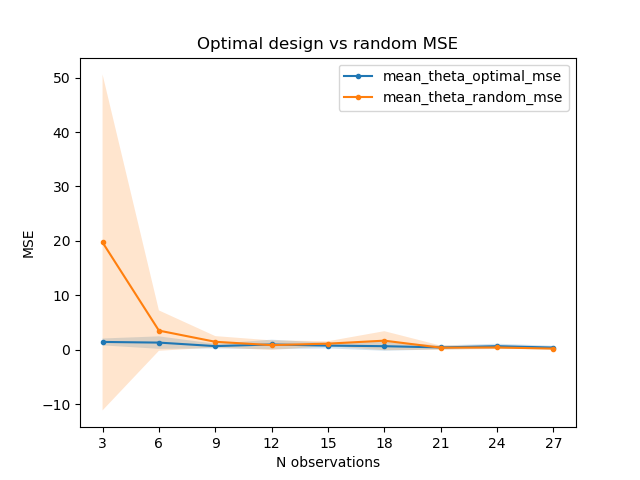
\includegraphics[scale=1.0]{heteroscedastic-experiment.png}
	\caption {График точности оценки параметров в зависимости от числа наблюдений}
	\label{fig:heteroscedastic-experiment}
\end{figure}

Таким образом $D$-оптимальный план позволяет существенно снизить число проводимых наблюдений при достижении той же точности оценок.


